\documentclass[../ms.tex]{subfiles}

\begin{document}

\begin{figure}
    \centering
    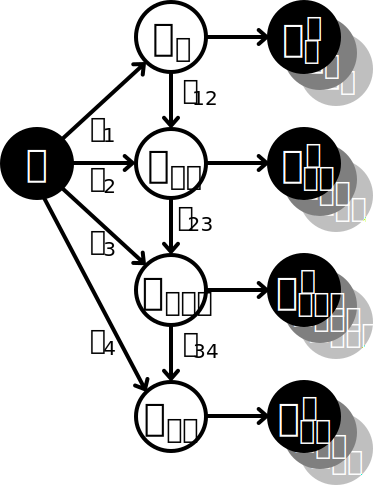
\includegraphics{figures/BN.pdf}
\end{figure}

We model the state of each \gls{lnl} as a hidden or unobserved binary random variable, which indicates via values 0 or 1 if an \gls{lnl} is healthy or involved, respectively. This state indicates if there is truly tumor present in an \gls{lnl}, including the presence of occult metastases for the involved state – motivating the term hidden or unobserved state. Every \gls{lnl} can be diagnosed using one or multiple modalities. Most used for diagnosis are imaging techniques like \gls{pet}, \gls{ct} and \gls{mri}, but palpation or \gls{fna} are also used. The diagnosis too, is modelled as binary random variable – this time an observed one – taking on 0 for negative and 1 for positive.

For notational convenience, we collect the hidden and observed random variables in a random vector each:
%
\begin{equation}
    \begin{aligned}
        \text{hidden}& & \mathbf{X} &= ( X_v ) \rightarrow \{ 0,1 \}^V \\
        \text{observed}& & \mathbf{Z} &= ( Z_v ) \rightarrow \left\{ 0, 1 \right\}^V
    \end{aligned}
\end{equation}
%
where $V$ is the number of \glspl{lnl} $v \in \{ 1,2,\ldots,V \}$ in the graph. The conditional probabilities that link the hidden state to the observations can be written as follows:
%
\begin{multline}
    P_{BN} \left( Z_v = z_v \mid X_v = x_v \right) = \left( z_v + (-1)^{z_v} \cdot s_P \right)(1 - x_v) \\ 
    + \left( (1 - z_v) + (-1)^{1 - z_v} \cdot s_N \right) x_v
\end{multline}
%
with $s_N$ and $s_P$ being the sensitivity and specificity of the used diagnostic method. For example, for the probability of a false negative observation, i.e. diagnostic modality misses the presence of tumor, we get
%
\begin{equation}
    P_{BN} \left( Z_v = 0 \mid X_v = 1 \right) = 1 - s_N
\end{equation}
%
Spread of the tumor through the lymphatic network is represented in this model by directed arcs to and between \glspl{lnl} as illustrated in \cref{fig:unilateral_graph}. We introduce an additional vertex to the graph representing the primary tumor, which we assume to be the only one. Directed arcs from the primary tumor to an \gls{lnl} represent direct spread of tumor cells from the primary tumor to the \gls{lnl}. These arcs are associated with parameters $b_v$ that we call base probabilities, and which indicate the probability that the tumor spreads directly to \gls{lnl} $v$. When \gls{lnl} $v$ receives efferent lymphatics from an upstream \gls{lnl} $r = \pa(v)$ -- which we call a \emph{parent} of $v$ -- this too is represented by a directed arc from \gls{lnl} $r$ to $v$. These arcs are associated with transition probabilities $t_e$, where $e$ enumerates the set of edges $\left\{ r \rightarrow v \mid v \leq V ; r = \pa(v) \right\}$ of size $E$. The resulting \gls{dag} is shown in \cref{fig:unilateral_graph}, comprising ipsilateral levels I, II, II, through IV, and will be used throughout this work. However, when more data of detailed \gls{lnl} involvement including additional levels becomes available and/or contralateral involvement, the model can be extended.

The parameters $b_v$ and $t_e$ associated with the directed arcs represent conditional probabilities, i.e. $b_v$ answers the question given that all parent nodes are healthy, how likely is it that the primary tumor spreads to node $v$? $t_e$ on the other hand, can answer the following question: Assuming no efferent spread from the primary tumor and given that all parent nodes, except the \gls{lnl} $r$ that corresponds to the connection $e$, are healthy, what is the likelihood of node $v$ becoming metastatic? The conditional probability for involvement of \gls{lnl} $v$ given the state of its parent nodes is then given by
%
\begin{equation}
    P_{BN} \left( X_v = x_v \mid X_{\pa(v)} = x_{\pa(v)}, b_v, t_e \right) = x_v + (-1)^{x_v} (1 - b_v) (1 - t_e)^{x_{\pa(v)}}
\end{equation}
%
We note here that this parametrization assumes the \gls{ici}, thereby allowing us to describe the model using only a few interpretable parameters. Dropping this assumption, a \gls{bn} can also be defined using \gls{cpt} that have columns for every possible combinations of parent states. However, with the increase of the number of parent nodes (causes) in the graph, the number of parameters in the respective \gls{cpt} would grow exponentially.

For the graph in \cref{fig:unilateral_graph} we can write down the parametrized \gls{cpt} in the following manner:
%
\begin{equation} \label{eq:bn_cpt}
    \begin{aligned}
        P_{BN} \left( X_v = 0 \mid X_{\pa(v)} = 0 \right) &= 1 - b_v \\
        P_{BN} \left( X_v = 1 \mid X_{\pa(v)} = 0 \right) &= b_v \\
        P_{BN} \left( X_v = 0 \mid X_{\pa(v)} = 1 \right) &= (1 - b_v) \left(1 - t_{\pa(v)v}\right) \\
        P_{BN} \left( X_v = 1 \mid X_{\pa(v)} = 1 \right) &= 1 - (1 - b_v) \left(1 - t_{\pa(v)v}\right) 
    \end{aligned}
\end{equation}
%
In case of a more general network, in which some \glspl{lnl} receive efferent lymphatics from multiple other \glspl{lnl}, \cref{eq:bn_cpt} can be generalised and the conditional probability of the hidden state becomes
%
\begin{multline}
    P_{BN} \left( X_v = x_v \mid \left\{ X_{\pa(v)} = x_{\pa(v)} \right\}, \left\{ t_{\pa(v)v} \right\} , b_v \right) \\
    = x_v + (-1)^{x_v} (1 - b_v) \prod_{p \in \pa(v)}{\left( 1 - t_{pv} \right)}^{x_{\pa(v)}}
\end{multline}
%
where we marginalized over all hidden variables $X$. Here we have assumed that each patient's diagnosis $\mathbf{z} = \left\{ z_v \mid v \leq V \right\}$ is complete, meaning that we have a diagnosis for each \gls{lnl}. The likelihood can then be used to infer the model parameters via maximum likelihood inference or sampling.

\end{document}